\chapter{Introdução}\label{ch:introducao}

Este trabalho de mestrado está inserido em um projeto de pesquisa sobre o
Paradigma Orientado a Notificações (PON), que é um novo paradigma de
desenvolvimento de sistemas computacionais \cite{doc_simao_2005}. As
materializações atualmente mais estáveis do PON para programação de
\textit{software} são os arquétipos ou \textit{frameworks} dele sobre linguagens
de programação correntes, como C++, C\#, Java, Akka e Erlang/Elixir.
Naturalmente, a elaboração de um \textit{framework} PON em uma dada linguagem
viabiliza nela uma nova abordagem para o desenvolvimento de programas, que é
justamente a orientação a notificações, visto que as linguagens são inicialmente
desenvolvidas de acordo com um ou mais paradigmas existentes
\cite{van_roy_2012}.

A proposta apresentada por este trabalho consiste no desenvolvimento de uma nova
e ímpar materialização do PON por meio de um \textit{framework} distinto,
utilizando o padrão C++20 da linguagem de programação C++. A intenção é manter o
desempenho de \textit{frameworks} desenvolvidos com padrões anteriores da
linguagem C++, como o padrão C++98 utilizado no caso do \textit{Framework} PON
C++ 2.0, e ter as vantagens de desenvolvimento obtidas com \textit{framework}
feitos em linguagens ditas modernas como C\# e Java. Neste sentido, propõem-se
ademais um conjunto de melhorias sobre as materializações atuais do PON na forma
de \textit{frameworks}, culminando em um novo arquétipo chamado
\textit{Framework} PON C++ 4.0.

Tais melhorias no âmbito do \textit{Framework} PON C++ 4.0 são inclusive
possibilitadas pela nova versão do C++ em voga (C++20) com novos conceitos e
recursos, como ponteiros inteligentes (\textit{smart pointers}),
\textit{variadic templates}, expressões \textit{fold} e expressões
\textit{lambda}. As melhorias são igualmente inclusive de orientação sistêmica,
fazendo particularmente a aplicação de conceitos de programação genérica e de
desenvolvimento orientado a testes. Ainda, os meios de se expressar código em
PON são facilitados no proposto \textit{Framework} PON C++ 4.0, aproximando-se
do alto nível da Linguagem de Programação do PON, a qual faz parte do estado da
arte, mas ainda não do estado da técnica.

Este capítulo primeiramente apresenta a contextualização dos principais
conceitos explorados ao longo do desenvolvimento do trabalho. Subsequentemente
são apresentadas as motivações, as justificativas e os objetivos que compõem a
proposta desse trabalho.

\section{Contextualização}

Nesta contextualização é introduzido o Paradigma Orientado a Notificações (PON)
sob a ótica de paradigmas de programação, assim como uma revisão básica de seus
conceitos de modo a prover o embasamento necessário ao entendimento desse
trabalho. Também na contextualização são apresentados os conceitos de
programação genérica e desenvolvimento orientado a testes, os quais foram
aplicados no desenvolvimento deste trabalho referente ao PON.

Em tempo, é natural que os trabalhos que exploram o PON apresentem uma revisão
sobre paradigmas de programação e, particularmente, sobre o PON. Portanto, para
o desenvolvimento desta sucinta revisão se aproveita e referencia os conteúdos
desenvolvidos anteriormente em outros trabalhos do grupo de pesquisa do PON da
UTFPR, salientando os trabalhos de Banaszewski
(\citeyear{msc_Banaszewski_2009}), Santos (\citeyear{msc_santos_2017}) e
Ronszcka (\citeyear{msc_Ronszcka_2012}, \citeyear{doc_ronszcka_2019}).

\subsection{Paradigmas de Programação Dominantes}

Um paradigma de programação é tido como um modelo ou método de se desenvolver
programas, seguindo modelos linguístico-matemáticos e, ademais, um determinado
conjunto de princípios. Os paradigmas são definidos de forma a resolver
determinados problemas, à luz dos seus modelos e princípios. Assim, cada
paradigma tem seu próprio conjunto de regras que o torna melhor ou pior na
resolução de cada problema em específico \cite{van_roy_2012}.

As regras definidas pelos paradigmas de programação ou mesmo desenvolvimento
servem como guia para o estabelecimento de padrões (\textit{e.g.}, de
programação e execução) e ferramentas de desenvolvimento de soluções nas
respectivas linguagens de programação e mesmo de projeto (ou \textit{design}).
Tais regras também servem como uma orientação aos desenvolvedores sobre como
estruturar melhor os seus programas e também projetos que os precedem
\cite{van_roy_2004}.

No tocante a programação, dentre os principais paradigmas de programação
destacam-se quatro, o Paradigma Procedimental (PP), Paradigma Funcional (PF),
Paradigma Orientado a Objetos (POO) e o Paradigma Lógico (PL)
\cite{scott_2000,watt_2004,brookshear_2006}. Esses paradigmas são referenciados
como Paradigmas Dominantes. Ainda, pode-se considerar que PP e POO fariam parte
de um paradigma maior chamado Paradigma Imperativo (PI), bem como PF e PL fariam
parte de um paradigma maior chamado Paradigma Declarativo (PD)
\cite{gabbrielli_2010}. Naturalmente, pode-se ter interseção dos subparadigmas
em PD e PI, salientando o subparadigma PF a título de exemplo.

%Em todo caso, o PP e o POO do PI e o PF e o PL do PD, são conhecidos como
%Paradigmas Dominantes por estarem bem estabelecidos e em pleno uso prático. Nas
%próximas seções, ainda que de maneira sucinta, apresenta-se estes paradigmas
%dominantes, bem como os emergentes, que surgem no processo de evolução da forma
%de programar

Em todo caso, o PP e o POO do PI e o PF e o PL do PD, são conhecidos como
Paradigmas Dominantes por estarem bem estabelecidos e em pleno uso prático.
Apesar de sua ampla utilização estes paradigmas ainda apresentam certas
deficiências, como a presença de redundâncias (estruturais e temporais) e a
tendência a acoplamento no PI. Essas deficiências também estão presentes no PD
em certa medida, pois ele utiliza mecanismos de execução que se baseiam em
buscas sobre elementos passivos\footnote{A Seção \ref{sec:paradigmas} apresenta
e discute em maiores detalhes os paradigmas mencionados.}. Normalmente, o PD é
implementado sob linguagens em PI, na sua forma usual ademais
\cite{msc_Banaszewski_2009,doc_ronszcka_2019}.

\subsubsection{Paradigma Dominantes vis-à-vis PI \& PD}

%Além dos subparadigmas de programação dominantes PI, POO, PF e PD, os
%subparadigmas emergentes também podem, em alguma medida,

Os paradigmas dominantes podem ser classificados como subconjuntos dos dois
paradigmas maiores, nomeadamente o PI e o PD \cite{msc_Banaszewski_2009}. Essa
relação entre os paradigmas nesta visão dada é ilustrada na Figura
\ref{fig:classificacao}. Essa divisão hierárquica é útil, ainda que imperfeita,
pois os paradigmas apresentam características em comum entre si, tendendo a
ficar mais perto de um paradigma dominante que de outro. Em suma, esta
classificação facilita comparações com relação a estas características em comum
\cite{doc_ronszcka_2019}.

\begin{figure}[!htb]
  \centering
  \caption{Classificação dos paradigmas de programação}
  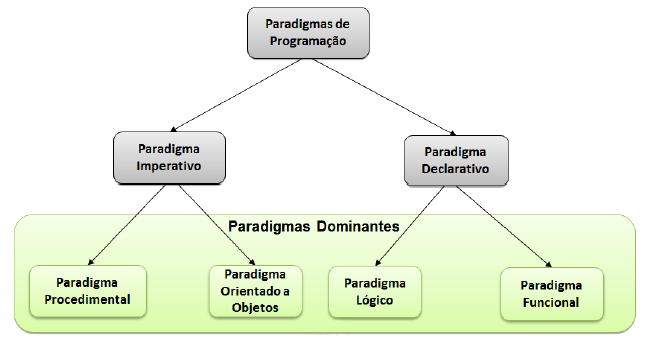
\includegraphics[width=0.85\textwidth]{../figures/classificacao_cut2.png}
  \caption*{Fonte: Adaptado de \citeonline{doc_ronszcka_2019}}
  \label{fig:classificacao}
\end{figure}

Segundo Peter Van Roy, cada paradigma tem seu conjunto de técnicas e conceitos
de programação que, conjuntamente, definem sua forma de estruturar o pensamento
na construção de programas \cite{van_roy_2012}. Com base nesses conceitos ele
elaborou uma taxonomia para paradigmas de programação, conforme apresentada na
Figura \ref{fig:paradigmas_roy}. Neste diagrama os paradigmas de programação são
organizados em um grafo que apresenta o relacionamento conceitual entre eles.
Neste contexto, setas entre dois quadros representando paradigmas representam a
adição de novos conceitos, de forma que o paradigma derivado contempla os
conceitos dos paradigmas anteriores, acrescidos de um ou mais novos conceitos
que, conjuntamente, os definem como paradigmas distintos \cite{van_roy_2012}.

\begin{figure}[!htb]
  \centering
  \caption{Taxonomia dos paradigmas e linguagens}
  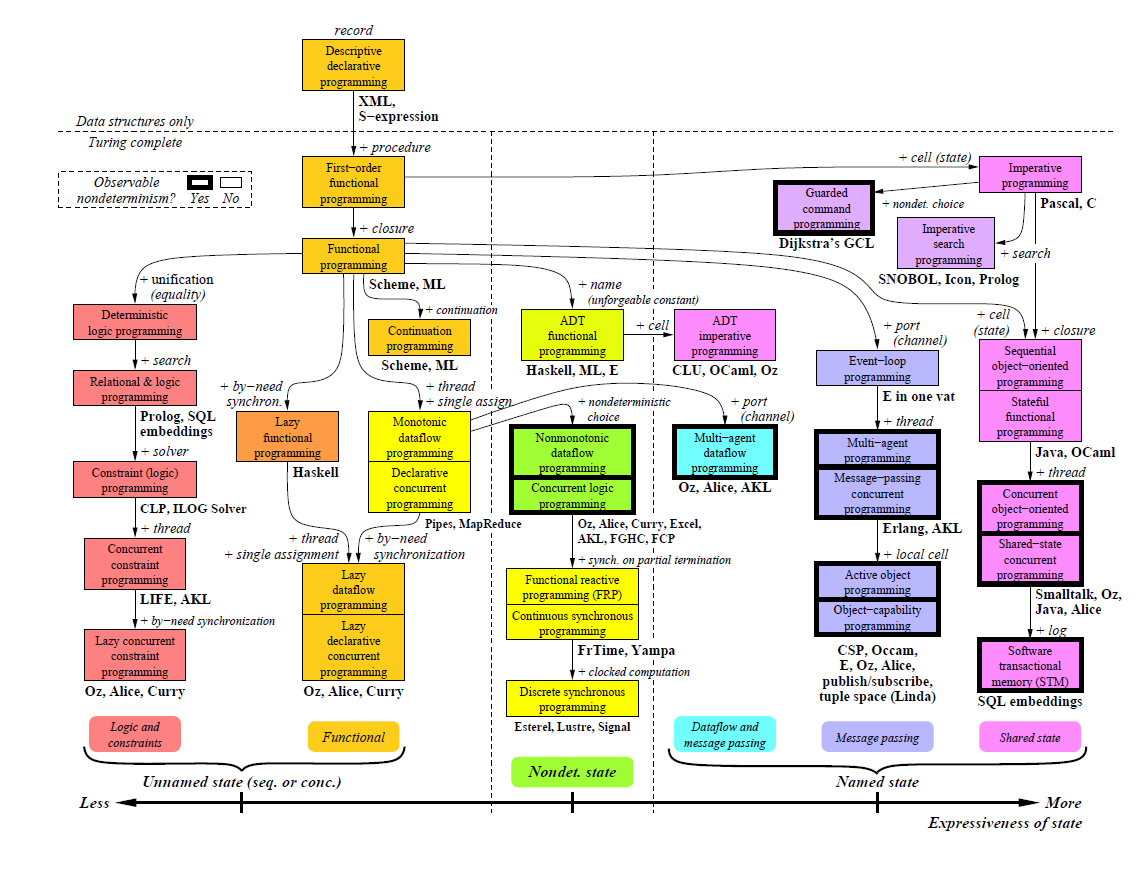
\includegraphics[width=\textwidth, height=0.46\textheight]{../figures/taxonomia.png}
  \caption*{Fonte: \citeonline{van_roy_2012}}
  \label{fig:paradigmas_roy}
\end{figure}

Cada linguagem de programação materializa um ou mais paradigmas, sendo que cada
paradigma é composto por um conjunto de conceitos \cite{van_roy_2012}. Essa
relação entre as linguagens, paradigmas e conceitos é ilustrada na Figura
\ref{fig:concepts}. Na prática, quanto mais paradigmas de programação uma
linguagem suportar, melhor seria, pois, em dados termos isso provê ao
desenvolvedor um conjunto ainda maior de ferramentas. Em havendo mais
ferramentas, elas podem ser escolhidas para serem utilizadas de forma a melhor
se encaixar no problema específico, visto que nenhum paradigma por si só seria a
melhor solução para todos os problemas \cite{van_roy_2004}.

Em verdade, no desenvolvimento de uma única aplicação podem sim, ser
encontrados diversos paradigmas, sendo eles aplicados em partes individuais do
programa e fidedignas a cada paradigma empregado. Esse estilo de programação é
naturalmente chamado de multiparadigma. Entretanto e finalmente, a utilidade de
uma linguagem multiparadigmas depende naturalmente de quão bem os diferentes
paradigmas estão integrados \cite{bjarne_1995,van_roy_2004}.

\begin{figure}[!htb]
  \centering
  \caption{Linguagens, paradigmas e conceitos}
  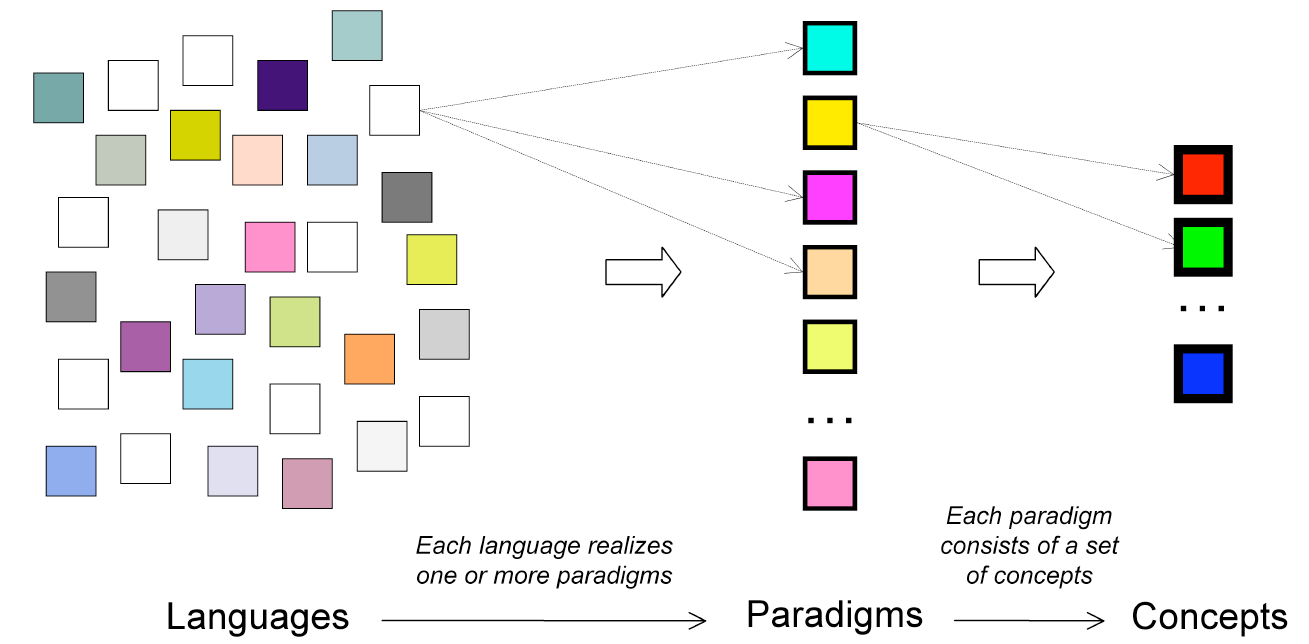
\includegraphics[width=0.85\textwidth]{../figures/concepts.png}
  \caption*{Fonte: \citeonline{van_roy_2012}}
  \label{fig:concepts}
\end{figure}

Dentre os paradigmas dominantes citados, o POO está entre os mais utilizados.
Essa conclusão pode ser tirada ao se observar o Quadro \ref{tab:linguagens}, em
que 4 das 5 linguagens mais populares em 2021 materializam o POO (Java, Python,
C++ e C\#), somando um total de 35,07\% no Índice TIOBE\footnote{A sigla TIOBE
  vem de \textit{The Importance of Being Earnest} (\textit{i.e.}, A Importância de
  Ser Zeloso), título de uma peça de comédia de 1895 de Oscar Wilde, que é a
  inspiração para nome da companhia holandesa homônima que mantém o Índice TIOBE.}
da Comunidade de Programação \cite{tiobe_2021}. Essas linguagens são as
conhecidas Java, Python, C++ e C\#.

Em tempo, o Índice TIOBE é um indicador de popularidade de linguagens de
programação, atualizado mensalmente, utilizando dados disponíveis nas
ferramentas de pesquisa online. Este índice não reflete qualitativamente sobre
as linguagens de programação, mas sim quantitativamente sobre o volume de código
escrito com as mesmas.

\begin{table}[!htb]
  \centering
  \caption{Índice TIOBE de linguagens de programação}
  \smallskip
  \begin{tabularx}{0.3\textwidth}{|X|l|}
    \hline
    Linguagem & Índice  \\
    \hline
    C         & 12,54\% \\
    \hline
    Python    & 11,84\% \\
    \hline
    Java      & 11,54\% \\
    \hline
    C++       & 7,36\%  \\
    \hline
    C\#       & 4,33\%  \\
    \hline
  \end{tabularx}
  \caption*{Fonte: Adaptado de \citeonline{tiobe_2021}}
  \label{tab:linguagens}

\end{table}

Além de suas vantagens técnicas, a dominância do POO entre os paradigmas pode
ser atribuída também aos sucessos comerciais das linguagens que os materializam,
à luz dos ganhos que a POO traz vis-à-vis ao PP, sendo justamente o PP o segundo
paradigma mais relevante neste mesmo índice de popularidade. Neste âmbito  do
domínio do POO, Java, C++ e Kotlin dominam o mercado de desenvolvimento Android,
enquanto Swift e Objective-C dominam o de iOS, de forma que é muito difícil
desenvolver \textit{software} para plataformas \textit{mobile} sem dominar o
POO. Da mesma forma, também tem se tornando importante conhecer o POO para o
desenvolvimento web, salientando aqui as linguagens JavaScript, Python e Ruby
\cite{gwosdz_2020}.

Dentre essas linguagens salientadas, destaca-se C++ em alguns aspectos, cuja
grande popularidade é atribuída por prover a velocidade de execução do C
enquanto dá suporte ao POO efetivamente, tendo permitido a transição do
PP para o POO por suportar ambos. De fato, desde a sua concepção, ela foi tida,
na verdade, como uma linguagem desenvolvida para suportar diversos estilos de
programação e, por sua vez, paradigmas, diferindo de linguagens que focam no
suporte de apenas um destes estilos \cite{bjarne_1995}. Com essa perspectiva de
ampliar o suporte a múltiplos paradigmas destaca-se a adição de expressões
lambda no padrão C++11, que ampliou o suporte do C++ ao paradigma de programação
funcional \cite{bjarne_2020}.

Mesmo uma linguagem como C++, entretanto, ainda herda os problemas de
sequencialidade da busca e orientação a pesquisas sobre elementos passivos por
meio de laços de repetição, advindo da computação sequencial. Na verdade, estes
problemas afetam desde linguagens imperativas até declarativas, sendo que estas
últimas, na prática, são implementadas com base nas primeiras finalmente,
conforme já discutido. Esses problemas trazem redundâncias temporais e
estruturais que podem causar prejuízos em desempenho e também em desacoplamento,
dificultando tanto a modularização do código como a execução de forma paralela
ou com paralelismos enfim, além da distribuída
\cite{simao_2009,simao_2012a,doc_ronszcka_2019}.

\subsection{Paradigmas de Programação Emergentes}\label{sec:intro_emergentes}

Conforme explicado anteriormente, o PP e o POO do PI e o PF e o PL do PD, são
conhecidos como Paradigmas Dominantes por estarem bem estabelecidos e em pleno
uso prático. Além dos Paradigmas Dominantes também existem diversos outros
paradigmas, ainda com menor grau de importância na prática industrial ou pelo
menos não ainda de mesmo impacto que os dominantes, dado que são propostas mais
recentes, mas que sim contribuem com novas formas de se conceber programas.

Estes novos paradigmas por sua vez são referenciados como Paradigmas Emergentes.
Dentre os Paradigmas Emergentes estão o Paradigma Orientado a Eventos (POE),
Paradigma Orientado a Componentes (POC), o Paradigma Orientado a Aspectos (POAs)
e o Paradigma Orientado a Agentes (POAg) \cite{msc_Banaszewski_2009}. A Figura
\ref{fig:emergentes} ilustra essa organização em Paradigmas Dominantes e
Emergentes, indicando justamente a precedência dos Paradigams Dominantes com
relação aos Paradigmas Emergentes.

\begin{figure}[!htb]
  \centering
  \caption{Classificação dos paradigmas de programação}
  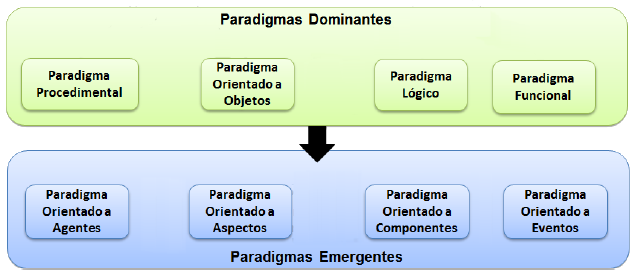
\includegraphics[width=0.85\textwidth]{../figures/classificacao_cut3.png}
  \caption*{Fonte: Adaptado de \citeonline{doc_ronszcka_2019}}
  \label{fig:emergentes}
\end{figure}

Os ditos Paradigmas Dominantes já estão estabelecidos há muito tempo, como o PP,
cuja origem foi na década de 50, enquanto os ditos Paradigmas Emergentes, em sua
maior parte, têm sua concepção mais recente, após a década de 90. Neste
contexto, a Figura \ref{fig:evolucao} apresenta uma linha temporal com os
Paradigmas Dominantes, exemplificando com as linguagens de programação nas quais
os paradigmas são aplicados e mesmo os Emergentes. Isto permite entender por quê
os Paradigmas Emergentes apenas iniciam sua trajetória para alcançar maior
impacto na prática industrial \cite{msc_Banaszewski_2009}.

\begin{figure}[!htb]
  \centering
  \caption{Evolução dos paradigmas de programação}
  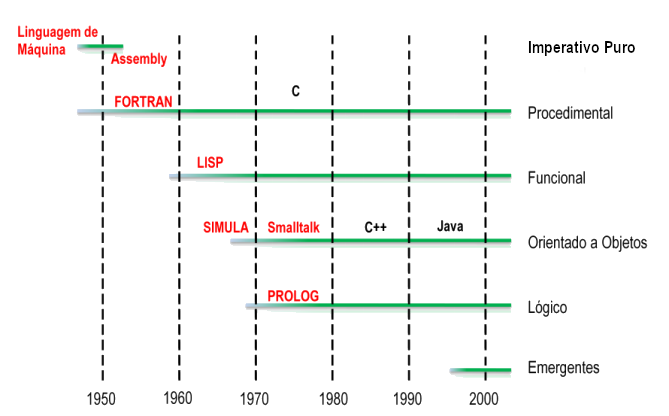
\includegraphics[width=0.8\textwidth]{../figures/evolucao.png}
  \caption*{Fonte: Adaptado de \citeonline{msc_Banaszewski_2009}}
  \label{fig:evolucao}
\end{figure}

Os ditos Paradigmas Emergentes citados buscam propor soluções a problemas
existentes dos Paradigmas Dominantes, porém ainda herdam os problemas de
sequencialidade pela orientação a buscas/percorrimentos do PI e POO, já
mencionados, ainda que atenuados em certa medida no Paradigma Orientado a
Eventos (POE), devido à interação entre objetos que ocorre por meio de eventos,
alterando o fluxo de execução do programa \cite{ferg_2006}. O detalhamento tanto
do POE como dos outros paradigmas mencionados neste capítulo é feito na Seção
\ref{sec:paradigmas}.

\subsection{Paradigma Orientado a Notificações — PON}\label{sec:pon}

À luz do apresentado nas seções anteriores, é introduzido o Paradigma Orientado
a Notificações (PON). O PON pode ser inserido nesse contexto como um paradigma
emergente, mas \textit{sui generis}. O PON surge embrionariamente em 2001 por
meio da proposta de um metamodelo para a solução de problemas de controle
discreto, o qual evoluiu como uma solução geral de inferência. Subsequentemente,
a solução evolui para um paradigma de programação e mesmo de desenvolvimento em
geral
\cite{simao_livro_2002,doc_simao_2005,pat_simao_2008,simao_2009,doc_ronszcka_2019}.
O PON, como paradigma de programação/desenvolvimento, tem os objetivos de tornar
menos árdua a tarefa do desenvolvimento de sistemas por permitir concepção em
alto nível, tornar o código e sua execução mais eficiente por evitar
redundâncias (estruturais e temporais) e, por fim, tornar a sua execução
paralelizável/distribuível por garantir o desacoplamento \cite{simao_2009}.

O PON até encontra inspirações no PI, tais como a flexibilidade algorítmica e a
abstração em forma de objetos do POO e mesmo a reatividade da programação
dirigida a eventos, entretanto ambas postas de modo distinto. Ele também
até aproveita conceitos próprios do PD, como a facilidade de programação em alto
nível e a representação do conhecimento em regras, mas também com as suas
próprias idiossincrasias que o permitem ser algo outro. Assim, neste âmbito, o
PON provê a possibilidade do uso de partes de ambos os estilos de programação em
alguma medida, apresentando, contudo, revoluções em seu modelo no tocante aos seus
constituintes, à organização deles e ao seu processo de inferência ou cálculo
lógico-causal \cite{pat_simao_2008,simao_2009,doc_ronszcka_2019}.

Como o próprio nome sugere, a principal característica estrutural do PON é que
ele é construído com base em notificações entre as suas entidades
(\textit{i.e.}, \textit{Attributes}, \textit{Premises}, \textit{Conditions},
\textit{Rules}, \textit{Actions}, \textit{Instigations} e \textit{Methods}),
havendo, portanto, um mecanismo para tal. Cada elemento constituinte do PON pode
enviar e/ou receber notificações pontuais, fazendo com que as avaliações lógicas
e causais somente sejam realizadas quando ocorre uma notificação. Na verdade, o
PON propõe a divisão da computabilidade em dois grandes grupos de entidades, um
grupo facto-execucional e outro grupo lógico-causal, relacionados entre si por
meio de notificações de seus constituintes. O primeiro grupo se constitui dos
\textit{Fact Base Elements} (\textit{FBEs}), enquanto o segundo se constitui em
entidades chamadas de \textit{Rules}.

Em suma, \textit{FBEs} e \textit{Rules} se compõem de elementos menores que
permitem realizar o fluxo de notificações entre \textit{FBEs} e \textit{Rules} e
vice-versa. No PON, cada \textit{Rule} é a entidade capaz de tratar uma
expressão lógico-causal. Assim, as \textit{Rules} gerenciam o conhecimento sobre
qualquer comportamento lógico-causal no sistema. O conhecimento lógico-causal de
uma \textit{Rule} provém normalmente de uma regra se-então, o que é uma maneira
natural de expressão deste tipo de conhecimento. Por sua vez, o \textit{FBE} é
uma entidade usada para descrever estados e serviços de entidades reais ou
cibernéticas em um problema computacional \cite{msc_Banaszewski_2009}.

Na Figura \ref{fig:nop_rule}, é apresentado um exemplo de entidade
\textit{Rule}, justamente na forma de uma regra lógico-causal, já com a
indicação de suas entidades constituintes menores \cite{neves_icist_2021}. A
\textit{Rule} ilustrada seria parte de um sistema de tomada de decisão relativa
a um dado sensor. Este sensor compõe a etapa facto-execucional do sistema na
forma de um \textit{FBE}, enquanto a \textit{Rule} compõe a etapa lógico-causal.

\begin{figure}[!htb]
  \centering
  \caption{Estrutura de \textit{Rule} no PON}
  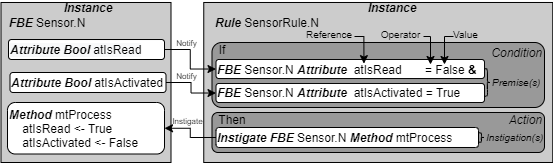
\includegraphics[width=0.95\textwidth]{../figures/rule_sensor_icist.png}
  \smallskip\smallskip\smallskip \caption*{Fonte: \citeonline{neves_icist_2021}}
  \label{fig:nop_rule}
\end{figure}

Mais precisamente, o sensor é representado pelo \textit{FBE} \textit{Sensor} com
seu \textit{Method} \textit{mtProcess} e seus \textit{Attributes}
\textit{atIsRead} e \textit{atIsActivated}. A \textit{Rule}, por sua vez,
apresenta uma \textit{Condition} que é composta por duas \textit{Premises} que
fazem as seguintes verificações sobre o \textit{FBE}: a) \textit{O sensor foi
  lido?} b) \textit{O sensor foi ativado?}. A aprovação desta \textit{Condition}
leva a execução da \textit{Rule}, que por sua vez aciona a sua \textit{Action},
a qual é composta uma \textit{Instigation}. A aprovação da \textit{Rule} resulta
na execução do \textit{Method} \textit{mtProcess} que implementa a
funcionalidade de processar no \textit{FBE Sensor}, atribuindo valores aos seus
\textit{Attributes} que levam a mudança de estado de cada um deles.

Em suma, a \textit{Condition} da \textit{Rule} em questão lida com a decisão de
processamento do sensor a partir de duas \textit{Premises} que avaliam estados
dos \textit{Attributes} do \textit{FBE Sensor}. Uma vez que a decisão seja
positiva, a \textit{Action} da \textit{Rule} é responsável pela instigação da
\textit{Instigation}, a qual instiga o \textit{Method} da \textit{Rule}. Isto
posto, por generalização, percebe-se que todo o processamento lógico-causal e
facto-execucional é efetuado por elementos constituintes das \textit{Rules} e
\textit{FBEs}, tidos como entidades pequenas ou mínimas
\cite{pat_simao_2008,simao_2009,doc_Kerschbaumer_2018}.

O diagrama de classes da Figura \ref{fig:nop_class} apresenta as relações entre
todos os elementos do chamado metamodelo do PON
\cite{simao_2009,msc_Ronszcka_2012,simao_2012a}. Assim sendo, cada um dos
elementos constituintes do PON é mais precisamente e mesmo sucintamente
detalhado conforme segue:

\begin{itemize}
  \item \textit{Fact Base Element} (FBE): Entidade de \textit{Elemento Base de
          Fatos} que contém os \textit{Attributes} e \textit{Methods}, podendo ser
        considerada similar aos objetos do POO em termos simplistas.
  \item \textit{Attribute}: Entidade de \textit{Atributo} que representa, cada
        qual, uma propriedade de um \textit{FBE}, sendo responsável por armazenar um
        valor discreto-factual que representa estados. Um \textit{Attribute} difere de
        uma variável do PP ou atributo do POO tradicional no sentido de que possui a
        capacidade de notificar \textit{Premises} relacionadas quando seu estado é
        alterado.
  \item \textit{Premise}: Entidade de \textit{Premissa} que realiza a avaliação
        lógica de estados de dois \textit{Attributes} por meio de determinado operador
        de comparação (\textit{e.g.,} igual, diferente, maior e menor) e notifica
        \textit{Conditions} relacionadas quando muda de estado lógico.
  \item \textit{Condition}: Entidade de \textit{Condição}, que realiza a
        avaliação lógica de \textit{Premises} por meio de determinado operador lógico
        (\textit{e.g.,} conjunção ou disjunção), e notifica \textit{Rules} relacionadas
        quando muda de estado, como de aprovada para reprovada e vice-versa.
  \item \textit{Rule}: Entidade de \textit{Regra}, relacionada a uma
        \textit{Condition}. Tipicamente, cada \textit{Rule} executa sua \textit{Action}
        quando é aprovada.
  \item \textit{Action}: Entidade de \textit{Ação}, cada \textit{Rule} é
        relacionada a uma \textit{Action}, que se relaciona com uma ou mais
        \textit{Instigations}. Ela ativa todas as suas \textit{Instigations} quando é
        executada uma vez notificada pela \textit{Rule}.
  \item \textit{Instigation}: Entidade de \textit{Instigação}, responsável por
        instigar os \textit{Methods} relacionados quando é ativada pela \textit{Action}
        relacionada.
  \item \textit{Method}: Entidade de \textit{Método} do PON, de forma análoga a
        funções membro (ou métodos) do POO, sendo executado quando notificado/instigado
        pela \textit{Instigation}.
\end{itemize}

%\begin{figure}[!htb] \centering
%\caption{Estrutura do
%\textit{FBE} no PON} 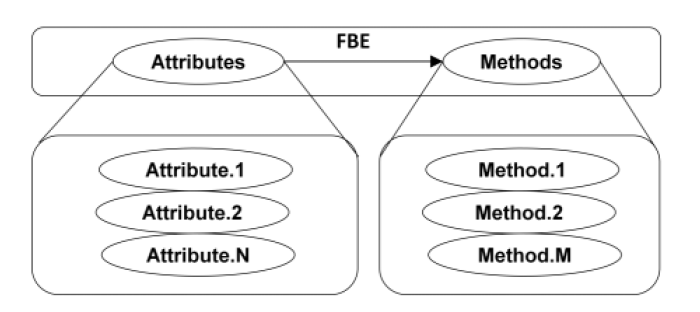
\includegraphics[width=0.6\textwidth]{../figures/fbe.png} \caption*{Fonte: \citeonline{msc_Banaszewski_2009}}
%\label{fig:fbe} \end{figure}

\begin{comment}

O diagrama de classes da Figura \ref{fig:nop_class} apresenta as relações entre
todos os elementos do metamodelo do PON
\cite{simao_2009,msc_Ronszcka_2012,simao_2012a}. À luz deste metamodelo, uma
\textit{Rule} é composta por uma entidade \textit{Condition} e uma entidade
\textit{Action}. A \textit{Condition} trata da decisão da \textit{Rule}, enquanto
a \textit{Action} trata da execução das ações da \textit{Rule}. Assim,
\textit{Condition} e \textit{Action} trabalham para realizar o conhecimento
causal da \textit{Rule}. Na verdade, tanto a \textit{Condition} quanto a
\textit{Action} são entidades reativas agregadas nela
\cite{simao_2009,simao_2012a,doc_ronszcka_2019}.

\end{comment}

\begin{figure}[!htb]
  \centering
  \caption{Diagrama de classes das entidades do metamodelo do PON}
  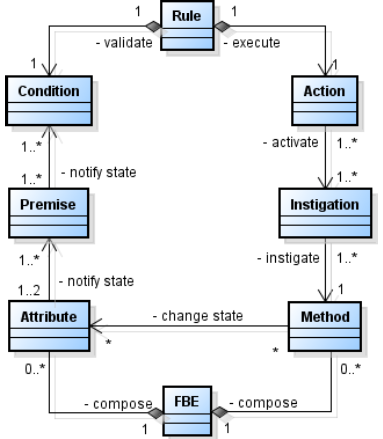
\includegraphics[width=0.6\textwidth]{../figures/metamodelo_pon.png}
  \caption*{Fonte: \citeonline{msc_Ronszcka_2012}}
  \label{fig:nop_class}
\end{figure}

O fluxo de execução, ilustrado na Figura \ref{fig:nop_chain}, ocorre em função
da mudança de estado de um \textit{Attribute} de determinado \textit{FBE}. A
mudança de estado no \textit{Attribute} notifica as suas \textit{Premises}, que
por sua vez reavaliam os seus estados lógicos. Se o valor lógico da
\textit{Premise} se altera ocorre então uma notificação para as
\textit{Conditions} interessadas no estado desta \textit{Premise}.
Consequentemente, cada \textit{Condition} avalia seu valor lógico segundo as
\textit{Premises} relacionadas. Quando a condição da \textit{Condition} é
satisfeita, isto resulta na aprovação da sua respectiva \textit{Rule} para a
execução. Quando a \textit{Rule} é aprovada, sua \textit{Action} é ativada. Uma
\textit{Action} é conectada a uma ou mais \textit{Instigations}, que por sua vez
acionam a execução de alguma funcionalidade de um \textit{FBE} por meio dos seus
\textit{Methods}. As chamadas para um \textit{Method} podem causar alteração nos
estados dos \textit{Attributes} e o ciclo de notificação recomeça
\cite{msc_Banaszewski_2009}.

O fluxo de iterações das aplicações em PON é realizado por meio de uma cadeia de
notificações pontuais entre as entidades do PON. Essa cadeia de notificações é
transparente ao desenvolvedor, porque as notificações são realizadas de forma
autônoma pelas entidades reativas do PON. O fluxo de iterações do PON difere do
fluxo de iterações de aplicações do PI, no qual o desenvolvedor deve modelá-lo
de maneira explícita por meio do uso de laços de repetição. No PON esse fluxo
acontece de forma natural na perspectiva de execução da aplicação, conforme
exemplificado na Figura \ref{fig:nop_chain} e esboçado no diagrama de classes da
Figura \ref{fig:nop_class}.

\begin{figure}[!htb]
  \centering
  \caption{Representação do fluxo de notificações do PON}
  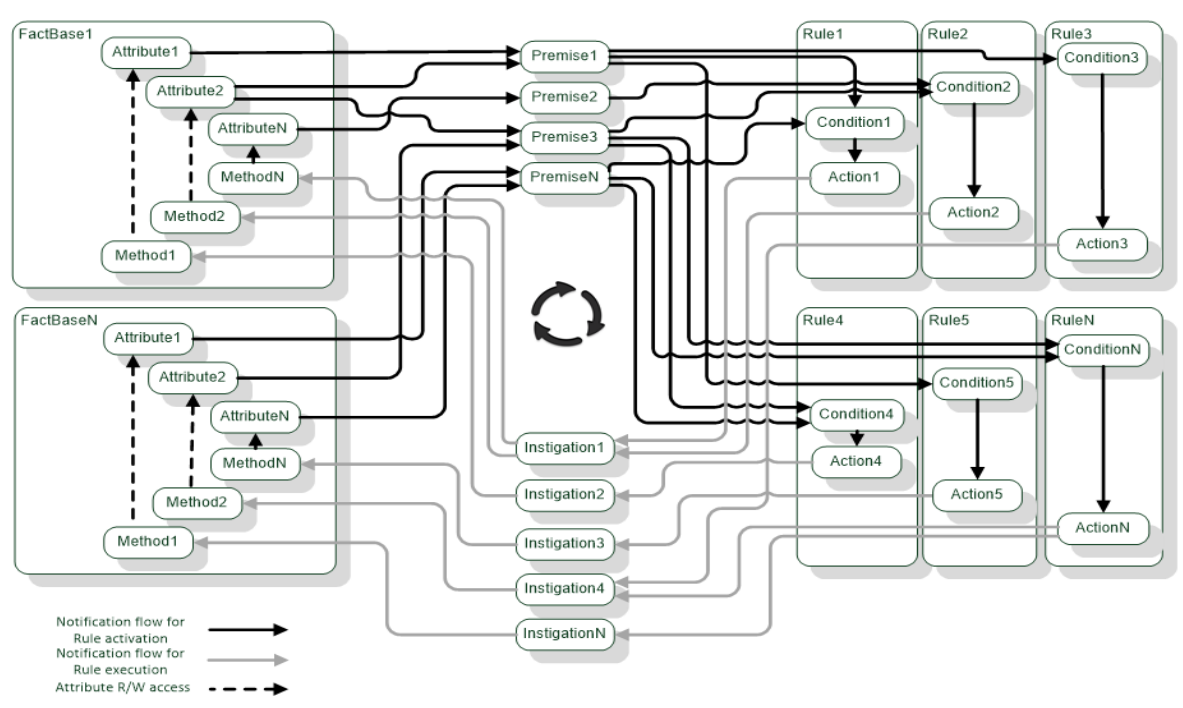
\includegraphics[width=\textwidth]{../figures/notificacoes_linhares.png}
  \smallskip
  \caption*{Fonte: \citeonline{doc_linhares_2015}}
  \label{fig:nop_chain}
\end{figure}

No PON, as entidades pequenas são reativas e efetivamente desacopladas, sendo
que colaboram entre si por meio de notificações pontuais de modo a realizar o
cálculo lógico-causal de forma precisa, nos termos já explicados, evitando
implicitamente redundâncias de processamento. Essas notificações ditam,
portanto, o fluxo de execução das aplicações. Eis que essa nova maneira de
concepção de programas tende a proporcionar melhora no desempenho das
aplicações, potencialmente facilitando a sua concepção, tanto para ambientes não
distribuídos como para ambientes distribuídos
\cite{pat_simao_2008,simao_2009,simao_2012a}.

Esta seção introduz o PON de maneira breve, sendo que nas Seções
\ref{sec:estado_arte_pon}, \ref{sec:review} e \ref{sec:conceitos_pon} é feita
uma revisão mais aprofundada do estado da arte do PON. Além disso, o PON não
está vinculado a nenhuma plataforma específica, possuindo implementações em
diversas plataformas. Uma revisão detalhada sobre as diversas materializações
disponíveis do PON é feita na Seção \ref{sec:frameworks}.

No tocante às implementações em plataformas de \textit{software},
particularmente dos \textit{frameworks}, uma lacuna destes é a falta de uso
extensivo de programação genérica, bem como a falta de orientação a testes
ostensiva nos seus desenvolvimentos. Nesse sentido, a Seção \ref{sec:generic}
apresenta os conceitos de programação genérica que podem ser aplicados em
materializações do PON.

\subsection{Programação Genérica}\label{sec:generic}

A programação genérica pode ser caracterizada como uma técnica de programação
que foca na abstração dos seus algoritmos na sua forma mais genérica, mas sem
perda de eficiência \cite{stepanov_2015}. A aplicação das técnicas de
programação genérica consiste em escrever código que consegue suportar e atender
adequadamente diferentes tipos de dados, no qual o tipo é interpretado como um
argumento que só é de fato aplicado quando o código for instanciado utilizando
um tipo concreto \cite{stepanov_1998}.

Essa técnica é frequentemente utilizada para resolver um problema inerente de
linguagens de programação com tipagem estática, que é a pouca flexibilidade de
tipos em comparação com as linguagens com tipagem dinâmica \cite{cardelli_1985}.
Nas linguagens com tipagem estática, os tipos das variáveis são resolvidos na
etapa de compilação, enquanto nas linguagens com tipagem dinâmica os tipos são
resolvidos apenas durante a execução. Tem-se como exemplo o C++ enquanto uma
linguagem com tipagem estática, bem como a linguagem Python enquanto uma
linguagem com tipagem dinâmica \cite{hurd_2021}.

Mais precisamente, um problema clássico que a programação genérica resolve é a
duplicidade de código, principalmente em linguagens com tipagem estática. É
muito comum haver a necessidade de realizar operações ou algoritmos, por meio de
funções, utilizando variáveis de diversos tipos ao longo do código. Um exemplo
usual são estruturas de dados, como listas encadeadas, que atuam sobre entidades
computacionais de diversos tipos. Nesse tipo de caso, pode haver a duplicação de
código ao declarar funções diferentes, ainda que similares, para o tratamento de
cada tipo \cite{alexandrescu_2001,stepanov_2015}.

Os códigos e algoritmos desenvolvidos com programação genérica precisam,
entretanto, alcançar um desempenho tão bom quanto algoritmos escritos com código
em tipagem específica, caso contrário seria muito difícil justificar seu uso em
casos nos quais o desempenho seja uma característica importante
\cite{stepanov_2015}. A substituição dos tipos em tempo de compilação faz com
que o compilador gere o código especializado para cada tipo instanciado pelo
programa, de forma que tanto o desempenho como as propriedades fornecidas pela
tipagem estática são mantidas mesmo em um quadro de código genérico
\cite{alexandrescu_2001}. Neste âmbito, caso o compilador tente instanciar o
código genérico utilizando um operador ou conversão não suportada pelo tipo
instanciado isso vai resultar em um erro de compilação \cite{bos_2019}.

No caso do C++ em particular, o principal recurso utilizado para a aplicação de
programação genérica são os \textit{templates}. Com os \textit{templates},
declara-se um tipo genérico, o qual é utilizado na definição do código em
desenvolvimento. Subsequentemente, o compilador se encarrega de substituir os
tipos conforme as chamadas deste código sejam instanciadas utilizando tipos
específicos. Essa substituição de tipos é feita na etapa de compilação, de forma
que isso não causa prejuízos em desempenho \cite{alexandrescu_2001}.

Tendo como exemplo uma função simples em C++ que retorna o máximo entre dois
valores, enquanto em uma implementação regular seria necessário criar código
dedicado para cada tipo utilizado, pode-se ter uma função genérica utilizando
\textit{templates}. Tais exemplos são mostrados nos Códigos
\ref{cod:getmax_regular} e \ref{cod:getmax_template}, respectivamente. É
interessante observar que na implementação do Código \ref{cod:getmax_regular} o
código utilizado no corpo das duas funções é igual, enquanto a
implementação do Código \ref{cod:getmax_template} elimina este código repetido.

\noindent
\begin{minipage}{.45\textwidth}
  \begin{lstlisting}[caption = {Função \textit{GetMax} sem \textit{templates}},
    source = {Autoria própria},
    label = {cod:getmax_regular}]
    int GetMax(int a, int b) {
      return (a>b)? a:b;
    }
    
    float GetMax(float a, float b) {
      return (a>b)? a:b;
    }
    
    int main() {
      GetMax(1, 2);
      GetMax(1.5, 2.7);
      return 0;
    }
    \end{lstlisting}
\end{minipage}\hfill
\begin{minipage}{.45\textwidth}
  \begin{lstlisting}[caption = {Função \textit{GetMax} com \textit{templates}},
    source = {Autoria própria},
    label = {cod:getmax_template}]
    template <typename T>
    T GetMax(T a, T b) {
      return (a>b)? a:b;
    }
    
    int main() {
      GetMax(1, 2);
      GetMax(1.5, 2.7);
      return 0;
    }
    \end{lstlisting}
\end{minipage}

Além da utilização de \textit{templates} para a passagem de argumentos de
funções, também é possível utilizar \textit{templates} na construção de classes.
Desta forma é possível definir os tipos de variáveis membros como
\textit{templates}, possibilitando a reutilização de código. No exemplo do
Código \ref{cod:template_class} são definidas classes para a implementação de
uma lista simplesmente encadeada com tipo genérico.

\begin{lstlisting}[caption = {Classe genérica com \textit{templates}},
source = {Autoria própria},
label = {cod:template_class}]
template <typename T>
class ListItem {
  // Definição da classe
  T* item;
  T* next;
}

template <typename T>
class List {
  // Definição da classe
  ListItem<T> head;
};

List<Animal> list_of_animals;
List<Car> list_of_cars;
\end{lstlisting}

Outro exemplo é apresentado no Código \ref{cod:ex_generic_1}, onde classes
distintas realizam um processo de inicialização por meio do método
\textit{init()}. Considerando uma situação na qual as classes A, B e C não são
relacionadas, de modo que não seria pertinente a aplicação de herança do POO, e
que os métodos \textit{init()} sejam similares, porém não idênticos, pode haver
duplicação de código nos métodos \textit{init()}. Neste caso pode ser feita a
aplicação de programação genérica para implementar parte destas funcionalidades
comuns, conforme apresentado no Código \ref{cod:ex_generic_2}. Desta forma, é
possível eliminar a duplicação de código desnecessária, sem haver quebra de
conceitos como herança \cite{thorsen_2015}. Em um programa sem a aplicação de
programação genérica seria necessário escrever o mesmo código duas vezes. Isso
traz o problema de duplicar o esforço gasto escrevendo código, assim como abre
espaço para o aparecimento de problemas futuros, pois a partir desse momento
será necessário fazer a manutenção de dois códigos separados. Portanto, podem
acabar surgindo defeitos em um ou outro, e eventualmente esses códigos podem
acabar divergindo e apresentando comportamentos diferentes, o que não seria o
desejado pela solução inicial \cite{stepanov_2015}.

\noindent
\begin{minipage}{.45\textwidth}
  \begin{lstlisting}[caption = {Exemplo de código sem programação genérica},
source = {Adaptado de \citeonline{thorsen_2015}},
label = {cod:ex_generic_1}]
class A {
    void init() {
        // Longo trecho de código complexo;
    };
};
class B { 
  void init() {
        // Similar ao init() de A 
  };
};
class C { 
  void init() {
        // Similar ao init() de A 
  };
};
\end{lstlisting}
\end{minipage}\hfill
\begin{minipage}{.45\textwidth}
  \begin{lstlisting}[caption = {Exemplo de código com programação genérica},
source = {Adaptado de \citeonline{thorsen_2015}},
label = {cod:ex_generic_2}]
template static inline void f1(T* t) {
    // Faz parte do trabalho de init()
    t->doSomething();
}
template static inline void f2(T* t) {
    // Faz outra parte do trabalho de init()
}
template static inline void f3(T* t) {
    // Faz outra parte do trabalho de init()
}
...
void A::init() {
	f1(this);
	f2(this);
	f3(this);
}
void B::init() { // Não utiliza f1
	f2(this);
	f3(this);
}
void C::init() { // Não utiliza f2
	f1(this);
	f3(this);
}
\end{lstlisting}
\end{minipage}

Na linguagem de programação C++ existe a biblioteca \textit{Standard Template
  Library} (STL), o que se constitui em um importante recurso nesta linguagem. A
STL é a biblioteca padrão de \textit{templates} que, dentre outros recursos,
contém definições de estruturas e algoritmos genéricos implementados com
\textit{templates}. Dentre esses, podemos citar as estruturas de listas,
vetores e algoritmos de ordenação e busca \cite{iso_cpp17}.

De forma geral, é dito que a programação genérica deve ser utilizada sempre que
possível, visto que reduz a duplicidade de código \cite{alexandrescu_2001}.
Porém, como contraponto, ela resulta em um código que é mais complexo, podendo causar
dificuldades para programadores iniciantes, que não tenham um domínio tão
completo da linguagem e que, portanto, apresentarão maior dificuldade em entender
essas construções genéricas mais complexas \cite{stepanov_2015}.

O suporte à programação genérica foi ampliado nas versões mais atuais do padrão
da linguagem de programação C++, com a adição de novos recursos, como
\textit{variadic templates} e \textit{fold expressions}
\cite{grimm_2020,bjarne_2020}. Em suma \textit{variadic templates} permitem a
utilização de \textit{templates} para a declaração de funções e métodos que
recebem um número variável de argumentos, enquanto as \textit{fold expressions}
fornecem os mecanismos necessários para se operar sobre esses conjuntos de
argumentos variáveis. Na Seção \ref{sec:cpp_moderno} são explorados com maiores
detalhes os recursos utilizados no escopo deste trabalho, incluindo
\textit{variadic templates} e \textit{fold expressions}.

Dado esse contexto é possível destacar que estes conceitos de programação
genérica podem ser aplicados no desenvolvimento dos \textit{frameworks} do PON
em C++ de modo a permitir maior flexibilidade de tipos e flexibilidade
algorítmica. A aplicação destes conceitos pode contribuir principalmente no
sentido de facilitar a programação em alto nível. A falta disto se constitui em
uma das imperfeições dos atuais \textit{frameworks} do PON. 

Outrossim, outra imperfeição seria a falta de ostensivo desenvolvimento
orientado a testes nos \textit{frameworks}. A carência da realização de testes
no processo de desenvolvimento das materializações atuais resulta em
dificuldades relativas ao seu uso principalmente no que diz respeito a presença
de problemas no código (\textit{i.e.}, \textit{bugs}) que são percebidos apenas
durante a sua utilização como, por exemplo, no caso do \textit{Framework} PON
C++ 2.0 conforme relatado por \citeonline{msc_xavier_2014} e no caso do
\textit{Framework} PON C++ 3.0 conforme relatado por
\citeonline{doc_Schutz_2019}

\subsection{Desenvolvimento Orientado a Testes — \textit{Test Driven
    Development} (TDD)}\label{sec:tdd_intro}

O método de desenvolvimento chamado Desenvolvimento Orientado a Testes ou, em
idioma inglês, o assim chamado \textit{Test Driven Development} (TDD), surgiu no
final da década de 90 \cite{test_driven_2013}, tendo seu ciclo de
desenvolvimento formal estabelecido por \citeonline{beck_2002}. O TDD é um
método que permite aumentar a confiabilidade do \textit{software}, por meio do
desenvolvimento de testes.

Como este presente trabalho envolve o desenvolvimento de um novo \textit{framework}
para PON em C++ (a chamada versão 4.0), inclusive com maior generalidade e
também com maior confiabilidade, há de se ter uma forma de reduzir o número
problemas encontrados durante seu uso e execução. Neste âmbito, a aplicação do
TDD se torna pertinente a este trabalho.

O uso de TDD evitaria enfim reincorrer em problemas no desenvolvimento de
\textit{frameworks} precedentes do PON, como erros de execução e retrabalho para
localizar a falha e alcançar as correções devidas. Por exemplo, há um erro
reportado no \textit{Framework} PON C++ 2.0 em \citeonline{msc_xavier_2014} que
só foi resolvido subsequentemente no \textit{Framework} PON C++ 3.0 em
\citeonline{belmonte_2012}, que por sua vez tinha imperfeições
tratadas apenas em \citeonline{doc_Schutz_2019}.

Isto dito, o método do TDD transforma o processo de desenvolvimento do
\textit{software}, dando maior foco ao desenvolvimento dos testes. Uma concepção
equivocada, porém muito comum, do TDD é que todos os testes devem ser
desenvolvidos de uma única vez no começo da etapa de desenvolvimento.
Entretanto, na aplicação correta deste método, é dado foco ao desenvolvimento de
um teste por vez \cite{test_driven_2013}.

No ciclo de desenvolvimento estabelecido pelo TDD tem-se em primeiro lugar o
desenvolvimento de um teste para a funcionalidade que se deseja implementar.
Inicialmente a execução deste teste deve falhar, visto que a funcionalidade
ainda não foi implementada. Após a falha inicial do teste é feita a
implementação do código e então os testes são executados novamente. Esse ciclo
se repete até que todos os testes passem e enfim pode ser dado início ao ciclo
de implementação de uma nova funcionalidade \cite{ambler_2006}. Esse fluxo é
ilustrado na Figura \ref{fig:tdd_flow}.

\begin{figure}[!htb]
  \centering
  \caption{Fluxo de desenvolvimento no TDD}
  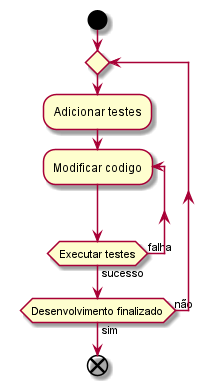
\includegraphics[width=.33\textwidth]{../out/diagrams/tdd/tdd.png}
  \smallskip
  \caption*{Fonte: Adaptado de \citeonline{mody_2017}}
  \label{fig:tdd_flow}
\end{figure}

Nesse contexto, o TDD recorre a dois tipos de testes, os testes unitários e
testes de integração \cite{ambler_2006}. Os testes unitários são aqueles que
avaliam o funcionamento de uma unidade do código (como classes, objetos ou
funções), enquanto os testes de integração avaliam o funcionamento de diferentes
partes do sistema operando juntas. Em todo caso, para ambos os tipos de teste,
aplica-se o ciclo ilustrado na Figura \ref{fig:tdd_flow}.

Um dos principais benefícios desse método é que, uma vez que os testes já foram
desenvolvidos, torna-se possível garantir que a implementação de novas
funcionalidades não altera as funcionalidades já existentes no sistema, que
foram previamente testadas, contanto que os testes continuem sendo executados
com sucesso. O TDD também ajuda o desenvolvedor a detectar problemas na
arquitetura do \textit{software} durante o desenvolvimento
\cite{test_driven_2013}.

Em contraponto aos benefícios anteriormente apresentados, uma das maiores
dificuldades para a adoção do TDD no processo de desenvolvimento de
\textit{software} é que os inúmeros ciclos de desenvolvimento de testes e
desenvolvimento de código tendem a aumentar significativamente o tempo de
desenvolvimento. Entretanto, certamente, esse tempo gasto na etapa de
desenvolvimento é compensado pelo tempo economizado corrigindo problemas de
código durante a execução do \textit{software} desenvolvido
\cite{test_driven_2013}.

Devido a esse grande número de iterações de testes que acontecem durante o
processo, é essencial que os testes sejam fáceis de executar e também rápidos,
pois caso isto não ocorra esse processo pode consumir muito tempo durante o
desenvolvimento, no limite inviabilizando TDD \cite{test_driven_2013}. Assim,
para auxiliar neste processo, existem diversas ferramentas que podem auxiliar o
desenvolvedor, sendo que na Seção \ref{sec:test_frameworks} são apresentados
\textit{frameworks} para a realização de testes em C++.

Em suma, a aplicação do TDD no contexto do desenvolvimento de um novo
\textit{framework} do PON é importante, pois, conforme já explicado, permite
garantir a estabilidade do \textit{software} desenvolvido. Isso contribui para
melhorar a experiência de uso do \textit{framework} e, por tanto, do paradigma,
pois reduziria significativamente o número de problemas encontrados durante o
uso do mesmo por outros desenvolvedores.

\section{Motivação}\label{sec:motiv}

% As características e propriedades do Paradigma Orientado a Notificações (PON)
% apresentadas na Seção \ref{sec:pon} são interessantes ao 

% Essas necessidades se apresentam como uma motivação para a materialização do
% PON \cite{doc_ronszcka_2019}.

Os sistemas computacionais estão se tornando cada vez mais complexos ao longo
dos anos, exigindo cada vez mais soluções em \textit{software} e
\textit{hardware} que atendam às suas necessidades \cite{chien_2011,
quali_pordeus_2020}. Dentre as principais demandas contemporâneas e históricas
do desenvolvimento de \textit{software} está o desenvolvimento de programas em
alto nível, utilizando ferramentas que facilitem o processo de desenvolvimento.
Ademais, em simultâneo, almeja-se que tais programas apresentem alto desempenho,
com baixos tempos de execução. Por fim, eles deveriam ainda se adequar a
arquiteturas de computação modernas, como é o caso de arquiteturas de computação
\textit{multicore}, de forma a aproveitar seu potencial de paralelismo
\cite{belmonte_2016}.

Do ponto de vista de \textit{hardware}, mais especificamente, houve substancial
evolução no aspecto da integração de circuitos, sendo que no desenvolvimento de
processadores integram-se múltiplos núcleos em uma única pastilha, o que se
constitui nos processadores \textit{multicore} justamente
\cite{asanovic_2009,chien_2011, quali_pordeus_2020}. Nesse âmbito, de modo a
atingir alto desempenho, é necessário que o desenvolvimento de \textit{software}
seja capaz de fazer proveito da capacidade de paralelismo oferecida por tais
processadores, \textit{i.e.}, paralelizando \textit{threads} com granularidade
apropriada para tal
\cite{henessy_2003,doc_linhares_2015,belmonte_2016,msc_negrini_2019}.

Nesse contexto todo, considerando as características apresentadas na Seção
\ref{sec:pon}, o PON se apresenta como uma alternativa viável para o atendimento
destas demandas contemporâneas e históricas do desenvolvimento de
\textit{software}. À luz de sua teoria, as materializações em PON podem ser
evoluídas e utilizadas de forma a permitir o desenvolvimento de
\textit{software} em alto nível e com alto desempenho. O desenvolvimento de
\textit{software} em PON pode trazer benefícios como redução dos custos em tempo
de desenvolvimento ao permitir a programação em alto nível, ao mesmo tempo que
apresentaria desempenho compatível ou superior ao das tecnologias atualmente
utilizadas. Ademais, o alto nível de desacoplamento das entidades computacionais
em PON seria um facilitador para fins de paralelismo e/ou distribuição
\cite{simao_2012a,ronszcka_2017,doc_ronszcka_2019}.

Durante os últimos anos, o PON vem apresentando muitas evoluções, tanto do ponto
de vista do estado da arte, com o refinamento dos conceitos que formam o
paradigma, assim como do ponto de vista do estado da técnica. Dentre as
evoluções técnicas, está o desenvolvimento de \textit{frameworks} que
possibilitam a aplicação do paradigma em diversas linguagens de programação como
C++ \cite{msc_Banaszewski_2009,msc_Ronszcka_2012}, Java \cite{henzen_2015}, C\#
\cite{henzen_2015,msc_oliveira_2019}, Elixir/Erlang \cite{msc_negrini_2019}, bem
como por meio de linguagens ainda prototipais de programação próprias ao PON no
âmbito da chamada Tecnologia LingPON \cite{doc_ronszcka_2019}. Esses trabalhos
do estado da arte/técnica são explorados com mais detalhes na seção
\ref{sec:estado_arte_pon}, sendo salientados os \textit{frameworks} por serem
versões assaz estáveis, constituindo o estado da técnica enfim.

Ainda no âmbito do estado da técnica, eis que o paralelismo, justamente uma das
principais características do PON, não é implementada em certas versões de
\textit{framework}, particularmente naqueles em C++ e tampouco naqueles em C\# e
Java \cite{doc_ronszcka_2019}. Mais precisamente, isto é bem o caso do
\textit{Framework} PON C++ 1.0 e também do contemporâneo \textit{Framework} PON
C++ 2.0. Ainda, mesmo no \textit{Framework} PON C++ 3.0, que justamente visava
paralelismo ao nível de \textit{thread}, isto não é adequadamente ou, ao menos,
estavelmente implementado \cite{doc_ronszcka_2019,doc_Schutz_2019}. Por outro
lado, \textit{frameworks} PON que tratam mais apropriadamente deste tipo de
paralelismo, como \textit{Framework} Akka e \textit{Framework} Elixir/Erlang,
usam linguagens de nível muito alto (orientada a atores) que não primam pelo
alto desempenho, como ocorreria se fossem feitos em C++
\cite{doc_ronszcka_2019,msc_negrini_2019,negrini_2019,negrini_2019_2}.

Assim sendo, uma versão nova de \textit{framework}, do PON que resolvesse
imperfeições dos precedentes e tivesse usabilidade melhorada, facilitaria o
aprendizado e aplicação dos conceitos deste paradigma emergente. Esta nova
versão também poderia potencialmente aumentar o volume e qualidade das
aplicações desenvolvidas neste paradigma, por meio da natural redução do tempo
de desenvolvimento necessário para utilizar o \textit{framework}. Para tal, mais
pontualmente, o novo \textit{framework} deve ser mais versátil, inclusive
facilitando a integração com bibliotecas e aplicações externas, permitindo o uso
de programação genérica e tendo sido desenvolvido à luz de TDD. Quanto maior for
a maturidade das materializações do estado da técnica em PON e maior for a
facilidade de uso, maior será também a viabilidade do PON, auxiliando assim que
este evolua do estágio de Paradigma Emergente, no sentindo de começar a alcançar
a transição para um paradigma estabelecido, quiçá um dia tornando-se um
paradigma vigente.

Ainda no que diz respeito ao desempenho das aplicações, as materializações do
PON carecem de aplicações bem definidas que sirvam como \textit{benchmark} bem
estabelecido, permitindo a realização de comparações entre os
\textit{frameworks} do PON e até mesmo com outros paradigmas. Nesse contexto,
\citeonline{quali_pordeus_2020} propõe a utilização de dois algoritmos
conhecidos, o \textit{Random Forest} (que se trata de um algoritmo de
aprendizagem de máquina) e o \textit{Bitonic Sort} (um algoritmo de ordenação),
que permitiram a avaliação do desempenho do PON em ambientes \textit{mono} e
\textit{multicore}. De modo similar, \citeonline{msc_negrini_2019} também propõe
a implementação de algoritmos para o controle automatizado de tráfego. Com esse propósito,
uma versão nova de \textit{framework} do PON deveria ser capaz de implementar
tais aplicações propostas, se beneficiando também da utilização de ferramentas
que permitissem garantir a confiabilidade e reprodutibilidade destes resultados,
como por meio do uso de \textit{frameworks} de teste.

\section{Justificativa}

A principal forma disponível e tecnologicamente estável para o desenvolvimento
de aplicações no PON ainda é por meio do uso de \textit{frameworks}. Dentre
todas as materializações de \textit{frameworks} do PON, aquela que apresenta
maior grau de maturidade e estabilidade é o \textit{Framework} PON C++ 2.0
\cite{ronszcka_2017}. Apesar de todos os esforços já realizados no
desenvolvimento dos \textit{frameworks}, inclusive no \textit{Framework} PON C++
2.0, estes \textit{frameworks} ainda possuem muitas imperfeições e mesmo
deficiências. Isto foi, em partes, supra considerado e relatado neste trabalho.

Apesar dos \textit{frameworks} PON em C++ entregarem, do ponto de vista
conceitual, toda a funcionalidade necessária para o desenvolvimento de
aplicações em PON, eles ainda apresentam algumas limitações importantes, como
verbosidade, baixa flexibilidade de tipos, baixa flexibilidade algorítmica, além
de particularmente não contemplarem todas as propriedades elementares do PON.
Neste sentido, o \textit{Framework} PON C++ 2.0 não contempla a propriedade de
paralelismo, enquanto a programação em alto nível não é plenamente possível
devido principalmente à excessiva verbosidade de expressão de código imposta por
ele. O \textit{Framework} PON C++ 3.0, por sua vez, tenta materializar a
propriedade de paralelismo ao nível de \textit{thread}, porém não o faz de
maneira satisfatória, apresentando diversos problemas de estabilidade, conforme
reportado em \citeonline{doc_Schutz_2019} e outros
\cite{martini_2019,doc_ronszcka_2019,msc_negrini_2019}.

Além dos \textit{frameworks} em C++, os demais \textit{frameworks} também ainda
não atendem de forma satisfatória as demandas mencionadas na Seção
\ref{sec:motiv}. Os \textit{frameworks} em Java/C\# são versões prototipais e
sem contemplar paralelismo, enquanto as materializações em Elixir/Erlang e Akka
contemplam paralelismo, mas não possuem o desempenho apropriado possibilitado
pelas linguagens de mais baixo nível. Neste contexto, as propriedades atingidas
pelos \textit{frameworks} do PON são resumidas no Quadro \ref{tab:demandas}.

Os \textit{frameworks} C++ 2.0, C++ 3.0 e Java/C\# possuem o melhor desempenho
dentre os \textit{frameworks} do PON. Em termos de tempo de execução, devido à
implementação dos \textit{frameworks} em geral usando estruturas de dados
baseadas em linguagens do \textit{POO}, isto gera sobrecarga ou
\textit{overheads} que distanciam esta implementação do PON de sua teoria, com
cálculos assintóticos na ordem de \(O(n)\) para o caso médio e \(O(n3)\) para o
pior caso. No caso dos \textit{frameworks}, em determinados cenários, o
desempenho ainda é inferior quando comparado a aplicações implementadas
diretamente no \textit{POO}. Entretanto, é justamente nos \textit{frameworks} em
C++ que, em geral, os resultados ficam próximos ao de POO, ainda que não sempre
o superando como prevê a teoria, mas sim mantendo programação em mais alto nível
e com alto nível de desacoplamento ademais
\cite{msc_Banaszewski_2009,msc_valenca_2012}.

\begin{table}[!htb]
  \centering
  \caption{Propriedades do PON materializadas pelos \textit{frameworks} do PON}
  \smallskip
  \begin{tabularx}{\textwidth}{|l||*{6}{X|}}\hline
    \diagbox{Propriedade}{\textit{Framework}} & C++ 2.0    & C++ 3.0    & Java/C\#   & C\# IoT    &
    Elixir                                & Akka                                                                        \\\hline\hline
    Programação em alto nível             &            &            &            & \checkmark & \checkmark & \checkmark \\ \hline
    Paralelismo                           &            & \checkmark &            & \checkmark & \checkmark & \checkmark \\ \hline
    Desempenho                            & \checkmark &            & \checkmark &            &            &            \\ \hline
  \end{tabularx}
  \caption*{Fonte: Autoria própria}
  \label{tab:demandas}
\end{table}

Dadas estas demandas, é possível constatar que existe a necessidade de uma
materialização que contemple essas demandas de forma mais satisfatória. Conforme
já salientado, os \textit{frameworks} em C++ tendem a ter melhor desempenho
quando comparado aos outros \textit{frameworks} do PON, entretanto ainda falta
neles maior facilidade de programação concorrente e distribuída, assim como de
programação genérica. Entretanto, parte das limitações e problemas existentes no
\textit{Framework} PON C++ 2.0 e \textit{Framework} PON C++ 3.0 podem ser
considerados decorrentes das limitações da tecnologia utilizada em suas
implementações, mais precisamente, o padrão C++98 da linguagem de programação
C++. Nesse âmbito, as inovações introduzidas nos padrões mais novos do C++,
principalmente o C++17 e C++20, podem contribuir para possibilitar o
desenvolvimento de um \textit{framework} capaz de atender a todas essas
demandas.

Dado ao excelente equilíbrio entre nível apropriado de abstração e desempenho
apropriado, o C++ é uma linguagem de programação apropriada para se realizar a
materialização do PON. Conforme constatado em \citeonline{tiobe_2021}, o C++
continua sendo uma linguagem de programação popular, ademais. Naturalmente, a
possibilidade de se utilizar o PON em uma linguagem de programação popular
facilitaria a aceitação dele por parte de novos desenvolvedores. Adicionalmente,
isto também permitiria a integração com outros programas e bibliotecas já
existentes em C++ e associados, de forma mais simples, assim possibilitando o
desenvolvimento de aplicações completas.

Ainda, apesar do C++ ser tradicionalmente uma linguagem de programação mais
usada no contexto da orientação a objetos, novos recursos adicionados nas suas
revisões mais recentes facilitam a programação funcional, por meio do uso das
expressões \textit{lambda} \cite{bjarne_2020}. Isto pode ser muito bem utilizado
em materializações do PON em C++  ara prover maior nível de flexibilidade de
programação (facto-execucional). Neste sentido de flexibilizações, com a
aplicação da programação genérica do C++ é possível atingir a flexibilidade de
tipos no \textit{framework}. Enquanto no \textit{Framework} PON C++ 2.0 se
precisava definir e implementar estruturas novas para cada tipo de dado a ser
utilizado (como \textit{int}, \textit{double}, \textit{string} e \textit{bool}),
em versão orientada a \textit{templates}/gabaritos seria possível utilizar
qualquer tipo de dado, pois as interfaces serão genéricas, não sendo necessário
código específico para implementar um tratamento diferente para cada tipo de
dado de entrada.

Outra melhoria que pode ser obtida ao se aplicar a programação genérica é
possibilitar reduzir a quantidade de código necessária para se compor o
\textit{framework} em si. Isso traz benefícios, como facilitar a manutenção do
código por outros desenvolvedores e/ou pesquisadores, possibilitando assim uma
melhor evolução do \textit{framework}. Facilitar-se-ia adicionar novos recursos
por não se fazer necessário reescrever uma grande quantidade de código. Ademais,
as contribuições da aplicação de programação genérica permitiriam ainda o
desenvolvimento de interfaces mais flexíveis e fáceis de utilizar, no sentido de favorecer a
programação em alto nível.

Por fim, com o C++17 também foram introduzidos mecanismos que facilitam a
programação concorrente, provenientes de mecanismos de execução paralela, como o
conceito de políticas de execução\footnote{As políticas de execução em C++
permitem especificar se a execução de algoritmos e laços de repetição deve ser
executada de forma sequencial ou paralela, esse conceito é explorado em maiores
detalhes na Seção \ref{sec:cpp_moderno}}. Esses mecanismos, enquanto recursos
nativos da linguagem, tornam transparente ao desenvolvedor a paralelização da
execução de \textit{threads} do \textit{software}, o que vai ao encontro do PON
no sentido de permitir \textit{threads} com granularidade fina. Esses recursos
permitiriam contornar a deficiência do \textit{Framework} PON C++ 3.0 no que diz
respeito à estabilidade, conforme reportado inclusive em
\citeonline{martini_2019}. Por agora serem recursos nativos da linguagem
C++, estes mecanismos naturalmente apresentam maior estabilidade que
implementações customizadas de paralelização, como a desenvolvida no
\textit{Framework} PON C++ 3.0.

Desta forma, em suma, observa-se que é factível o desenvolvimento de uma versão de
\textit{framework} em C++ melhor que atenda as propriedades do PON e, portanto,
vá ao encontro de todas as demandas de desenvolvimento de \textit{software} supra
apresentadas. Em suma, a programação genérica poderia ser utilizada para
facilitar a programação em alto nível, o bom desempenho já observado nas
materializações de \textit{frameworks} do PON em C++ existentes seria mantido e
quiçá melhorado e, por fim, as políticas de execução poderiam ser utilizadas
para implementar o suporte ao paralelismo de forma simples e estável.

Apesar da maturidade e estabilidade apresentadas pelo \textit{Framework} PON C++
2.0, as limitações impostas pelas tecnologias utilizadas em sua implementação,
como o antigo padrão C++98 da linguagem C++, a excessiva verbosidade e grande
quantidade de código redundante dificultam a implementação de melhorias sobre
sua base de código. Desta forma, em suma, há espaço para a implementação de uma
nova materialização de \textit{framework}, a qual deve ser desenvolvida fazendo
proveito dos avanços no estado da técnica introduzidos pelos \textit{frameworks}
já disponíveis, porém realizando implementações mais apropriadas em termos de
programação contemporânea de \textit{software} aplicando as melhorias acima
propostas.

Além disso, a implementação de determinadas aplicações, como os
\textit{benchmarks} propostos por \citeonline{pordeus_2020} por meio dos
algoritmos \textit{Random Forest} e \textit{Bitonic Sort} são difíceis, ou quiçá
impossíveis, de serem implementados de forma satisfatória com o
\textit{Framework} PON C++ 2.0. O \textit{Random Forest} é um algoritmo de
aprendizagem de máquina, que pode se beneficiar da paralelização da execução de
suas árvores de decisão, o que não seria contemplado por implementações com o
\textit{Framework} PON C++ 2.0. Por sua vez, o \textit{Bitonic Sort} é um
algoritmo de ordenação, sendo composto por várias etapas de decisão avaliando
elementos dois a dois, que podem ser implementadas por várias \textit{Rules} do
PON, o qual seria difícil de implementar com o \textit{Framework} PON C++ 2.0
devido à complexidade da inicialização de suas entidades. Nesse sentido, a
implementação de um novo \textit{framework} do PON possibilitaria a realização
destes \textit{benchmarks}.

\section{Objetivo geral}\label{sec:obj_geral}

O objetivo geral deste trabalho é promover avanços ao Paradigma Orientado a
Notificações (PON) via um novo \textit{framework} orientado a TDD, programação
genérica e recursos modernos da linguagem de programação C++20 (\textit{single
thread} e \textit{multithread}), para melhor contemplar as propriedades
elementares do PON no estado da técnica, o que deve ser validado via
\textit{benchmarks} apropriados (\textit{e.g.}, \textit{biotonic} e
\textit{random forest}).

\section{Objetivos específicos}\label{sec:obj_especificos}

Para atingir o objetivo geral, este trabalho apresenta os seguintes objetivos
específicos:

\newcommand{\SubItem}[1]{
    {\setlength\itemindent{15pt} \item[-] #1}
}
\begin{itemize}
  %\item Dissertar sobre as materializações do PON, fazendo as devidas críticas
  %(como a falta de programação genérica e \textit{multithread} efetivo em
  %materializações em C++) e propondo melhorias a serem contemplados na nova
  %versão de \textit{framework} PON C++. \item Realizar um levantamento de
  %técnicas de programação em C++ moderno, com a utilização das funcionalidades
  %adicionadas nos padrões C++11, C++14, C++17 e C++20, salientando as técnicas
  %de programação genérica e possibilidade de programação concorrente visando
  %\textit{multithread}.
  \item Desenvolver uma nova versão de \textit{framework} em C++, denominado
        \textit{Framework} PON C++ 4.0, tendo como base o \textit{Framework} PON
        C++ 2.0 enquanto estado da técnica e considerando as melhorias
        apresentadas nos demais \textit{frameworks} do PON.
  \item Prover as seguintes melhorias centrais sobre o \textit{Framework} PON C++ 2.0:
  \begin{enumerate}[label=(\alph*)]
  \item Adicionar a flexibilidade de tipos aos \textit{Attributes};
  \item Adicionar flexibilidade algorítmica às \textit{Conditions};
  \item Reduzir a verbosidade da utilização do \textit{framework};
  \item Permitir execução com paralelismo.
  \end{enumerate}
  \item Validar o \textit{framework} desenvolvido por meio de técnicas de teste
        no âmbito do desenvolvimento orientado a testes (TDD — \textit{Test
        Driven Development}).
  \item Desenvolver aplicação de simulação de sistema de sensores, oriunda do
        grupo de pesquisas do PON, para avaliar o desempenho do
        \textit{Framework} PON C++ 4.0 em ambientes \textit{monocore},
        comparando com o desempenho das implementações com o \textit{Framework}
        PON C++ 2.0 e com o POO em linguagem C++.
  \item Desenvolver aplicação com os algoritmos \textit{Bitonic Sort} e
        \textit{Random Forest}, oriundos da literatura, para avaliar o
        desempenho do \textit{Framework} PON C++ 4.0 em ambientes monocore
        vis-à-vis o PP em linguagem C, bem como para balanceamento de carga em
        \textit{multicore}.
  \item Desenvolver aplicação de simulação de controle de tráfego automatizado,
        oriunda do grupo de pesquisas do PON, para a avaliar o desempenho do
        \textit{Framework} PON C++ 4.0 em ambientes \textit{multicore},
        comparando com o desempenho das implementações com o \textit{Framework}
        PON Erlang/Elixir.
  \item Desenvolver aplicação sob a forma de um jogo para avaliar a utilização
        do \textit{Framework} PON C++ 4.0 em integração com bibliotecas externas
        (\textit{i.e.}, Unreal Engine) em linguagem de programação C++.

\end{itemize}

\section{Organização do trabalho}

Estra trabalho está dividido em cinco capítulos, incluindo este capítulo de
introdução. No Capítulo \ref{ch:arte} é feita uma revisão do estado da arte das
tecnologias utilizadas no desenvolvimento deste trabalho, apresentando de forma
sucinta as materializações do PON, ferramentas de C++ moderno e ferramentas de
teste. No Capítulo \ref{ch:desenvolvimento} é apresentado o desenvolvimento
realizado neste trabalho. Mais precisamente, é apresentada a modelagem do
\textit{Framework} PON C++ 4.0 proposto. O capítulo \ref{ch:result}, por sua
vez, apresenta os resultados de experimentos realizados com o objetivo de
avaliar o \textit{Framework} PON C++ 4.0 desenvolvido. Por fim, o Capítulo
\ref{ch:conclusao} apresenta as conclusões sobre este trabalho, assim como
explora as perspectivas para trabalhos subsequentes no âmbito da aplicação do
\textit{Framework} PON C++ 4.0.

